\documentclass{beamer}
\usepackage[utf8]{inputenc}
\usepackage[russian]{babel} 
\usepackage{amsmath,mathrsfs,mathtext}
\usepackage{graphicx, epsfig}
\usepackage{multirow}
\usepackage{booktabs}
\usepackage{bookmark}
\usepackage{bibentry}

\usetheme{Warsaw}%{Singapore}%{Warsaw}%{Warsaw}%{Darmstadt}
\usecolortheme{sidebartab}
\definecolor{beamer@blendedblue}{RGB}{15,120,80}
\beamertemplatenavigationsymbolsempty
\DeclareMathOperator*{\argmax}{argmax} 
%----------------------------------------------------------------------------------------------------------

%----------------------------------------------------------------------------------------
%	TITLE PAGE
%----------------------------------------------------------------------------------------
\title[\hbox to 56mm{DTW  \hfill\insertframenumber\,/\,\inserttotalframenumber}]
{Динамическое выравнивание многомерных временных рядов}
\author{Моргачев Г., Смирнов В., Липницкая Т.}
\institute{Московский физико-технический институт}
\date{\footnotesize{
\par\emph{Курс:} Автоматизация научных исследований в машинном обучении\par (практика, В.В. Стрижов)/2019
\par\emph{Консультант:} Гончаров А.
\date{\today}
}}
% \date{\today}
\begin{document}

%------------------------------------------------

\begin{frame}
\titlepage 
\end{frame}

%------------------------------------------------

\begin{frame}
\frametitle{Выбор функции расстояния}
\framesubtitle{при класстеризации и поиске паттернов в многомерных временных рядах}
    \begin{block}{Цель работы}
        Исследовать влияние выбора функции расстояния между векторами на 
        качество алгоритма DTW.
    \end{block}
    \begin{block}{Проблема}
        При обобщении метода выравнивания временных рядов на многомерный случай остается 
        открытым вопрос определения расстояния между парами векторов.
    \end{block}
    \begin{block}{Метод решения}
        Рассмотрение задач кластеризации и поиска паттернов для нахождения функции расстояния,
        позволяющей достичь на данных задачах наилучшего качества.
    \end{block}
\end{frame}


\begin{frame}
\frametitle{Многомерное выравнивание рядов}
    \begin{block}{}
        DTW: функция расстояния, учитывающая выравнивание рядов относительно сдвигов и сжатий.
        Использует расстояние между точками. 
    \end{block}    
    \begin{figure}
        \begin{columns}

            \column{0.65\linewidth}
               \centering
               Одномерный случай
               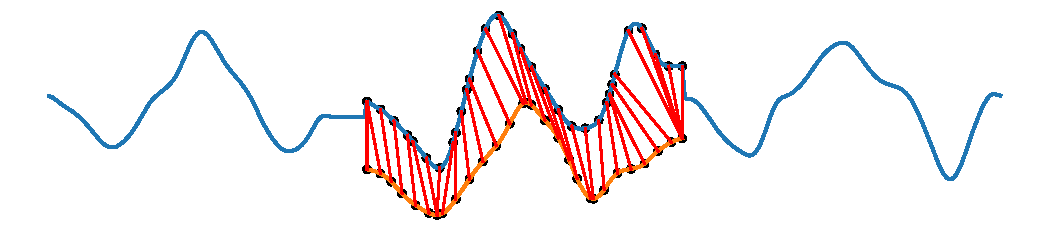
\includegraphics[width=\linewidth]{img1.pdf}
            \column{0.45\linewidth}
            \begin{itemize}
                \item  $S_1^i, S_2^i$ \-- числа
                \item  $\rho(S_1^i, S_2^i) = | x - y |$
            \end{itemize}
        \end{columns} 
        \begin{columns}
            \column{0.65\linewidth}
                \centering
               Многомерный случай
               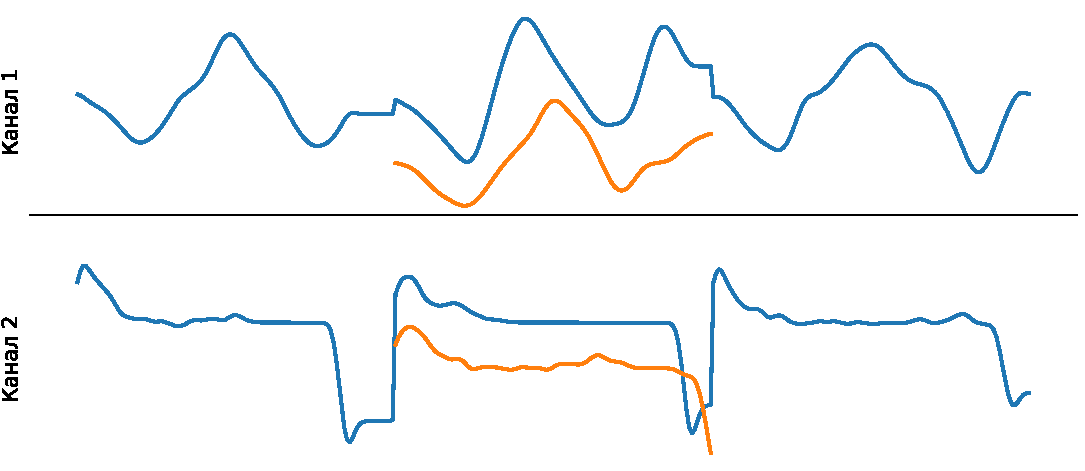
\includegraphics[width=\linewidth]{img2.pdf}
            \column{0.5\linewidth}
            \begin{itemize}
                \item  $S_1^i, S_2^i $ \-- вектора
                \item  $\rho(S_1^i, S_2^i) = \|S_1^i - S_2^i\|_1$
                \item  $\rho(S_1^i, S_2^i) = \|S_1^i - S_2^i\|_2$
                \item  $\rho(S_1^i, S_2^i) = \text{cos\_dist}(S_1^i, S_2^i)$          
            \end{itemize}

        \end{columns} 
    \end{figure}
\end{frame}    


\begin{frame}
\frametitle{Литература}
\bibliographystyle{alpha}
\nobibliography{literature} 
    Одномерный случай:
    \begin{enumerate}
        \item\bibentry{Rakthanmanon:2012:SMT:2339530.2339576}
    \end{enumerate}
    Многомерные обобщения:
    \begin{enumerate}
        \item\bibentry{Sanguansat2012MultipleMS}
        \item\bibentry{Holt2007}
    \end{enumerate}
\end{frame}
%------------------------------------------------

\begin{frame}
\frametitle{Постановка задачи}
    \begin{block}{}
        Дано множество $\boldsymbol{S}$ $l$\--мерных  временных рядов длины $n$. $S_i = \{s_i^1 \dots s_i^n\},\ S_i \in \boldsymbol{S},\ s_i^j \in \mathbb{R}^l$.\\
        Задано множество функций расстояния между векторами:
        $$\mathrm{R} = \{\rho: \mathbb{R}^l \times \mathbb{R}^l \rightarrow \mathbb{R}_+ \},$$
        $$\text{DTW}_{\rho}: \boldsymbol{S} \times \boldsymbol{S} \rightarrow \mathbb{R}_+.$$
    \end{block}

    \begin{block}{Общая постановка задачи}
        Для задач кластеризации и поиска паттернов вводятся соответствующие функции качества $Q_i$*.
        Рассматривается поиск оптимального $\rho$.
        $$
            \rho_i = \argmax_{\rho} Q_i(\rho)
        $$
    \end{block}
\end{frame}

\begin{frame}

    \begin{block}{Задача кластеризации}

        Для всех $S_i \in \boldsymbol{S}$ задано ${y_i \in \mathbb{Y}}$\---множество меток классов.
        Задана матрица попарных расстояний:
        $$D(\text{DTW}_\rho(\boldsymbol{S})) = ||D_{ij}||, \ \ D_{ij} = \text{DTW}_\rho(S_i, S_j),\ \ S_i, S_j \in \boldsymbol{S}.$$
        Модель кластеризации: $f: D \rightarrow Z^N$,\\ Z \-- множество меток кластеров.

    \end{block}

    \begin{block}{Метод класстеризации}
        \textbf{Иерархическая} с функциями расстояния между кластерами: 
        \begin{enumerate}
            \item \textit{complete:}  $d(A, B) = \max\limits_{a \in A, b \in B}(dist(a, b))$ 
            \item \textit{weighted:}  $d(A,B) = \dfrac{(dist(S,B) + dist(T,B))}{2}$, где кластер $A = S \cup T$
            \item \textit{average:}   $d(A,B) = \sum\limits_{a \in A, b \in B} \dfrac{d(a, b)}{(|A|*|B|)}$ 
        \end{enumerate} 
    \end{block}
\end{frame}

\begin{frame}
    \begin{block}{Функции качества кластеризации}
        \begin{align*}
            Q_1(\rho) = \frac{1}{|Z|}\sum\limits_{z \in Z} \max_y \frac{N_z^y}{N_z},\  Q_2(\rho) = \frac{1}{|Z|}\sum\limits_{z \in Z} \max_y \frac{(N_z^y)^2}{N_z N^y}.
        \end{align*}
        \begin{itemize}
            \item $N_z$ \-- количество элементов в кластере с меткой $z$. 
            \item $N^y$ \-- количество элементов в классе $y$.
            \item $N_z^y$ \-- количество элементов класса $y$ в классе $z$.
        \end{itemize}
    \end{block}
\end{frame}

\begin{frame}
    \begin{block}{Задача поиска паттернов}
        Задан временной ряд $S$ длинны $n$, содержащий сегменты класса $\boldsymbol{P}$. \\
        $\boldsymbol{P}$ \-- временные ряда длины $m \ll n$. \\
        Известны представители класса $\boldsymbol{P}$, необходимо найти участки $S$,
            соответствующие данному классу. \\
        $\boldsymbol{T} = \{t_1, \dots, t_j \}$ \-- множество начал таких событий. \\
        Участок найден, если пересечение с предполагаемым более $80\%$ от $m$.
    \end{block}

    \begin{block}{Функция качества поиска шаблонов}
        \begin{align*}
            Q_3(DTW_{\rho}) = \dfrac{\sum\limits_{i=1}^j [t_i \-- \text{найден}]}{j}.
        \end{align*}
    \end{block}
\end{frame}


%------------------------------------------------
 
\begin{frame}
    \frametitle{Эксперимент}   
    \begin{block}{Цель}
        Изучить зависимость качества кластеризации и поиска паттернов от выбора функции расстояния между векторами,
        при различных методах определения расстояния между кластерами и получения среднего ряда.
    \end{block}

    \begin{block}{Данные: класстеризация}
        \begin{itemize}
            \item Размеченные данные ускорений акселерометра телефона: 6 состояний человека,
                3 канала, разбиты по 50 точек.
        \end{itemize}
    \end{block}

    \begin{block}{Данные: поиск паттернов}
        \begin{itemize}
            \item Данные ECG: 4 состояния человека, 3 канала, разбиты на ряды по 206 точек.
            \item Написание букв: 20 символов, 3 канала, разбиты по 182 точки.
        \end{itemize}
    \end{block}
\end{frame}
    
%------------------------------------------------

\begin{frame}
    \frametitle{Результаты: поиск паттернов}   
    \begin{center}
        \begin{table}
            \begin{tabular}{c|c *{2}{|*{3}{c}}}  
                \toprule
                  \multirow{2}{*}{$\rho$}& \multirow{2}{*}{average} & 
                            \multicolumn{3}{c|}{characters} & \multicolumn{3}{c}{epi} \\
                \cmidrule(r){3-8}
                                   &  & $Q$ & $t$ & $t_{\text{no optim}}$ & $Q$ & $t$ & $t_{\text{no optim}}$ \\
                \midrule
            \multirow{2}{*}{$L_1$} 
                    & DBA    &   0.866   &   2.117   &    10.064   &   0.744   &   14.335   &    13.064\\
                    & mean   &   0.901   &   2.524   &    10.819   &   0.744   &   13.541   &    13.912\\
            \midrule        
            \multirow{2}{*}{$L_2$} 
                    & DBA    &   0.831   &   1.308   &     9.628   &   0.687   &   12.342   &    13.205\\
                    & mean   &   0.864   &   1.255   &    10.495   &   0.687   &   14.199   &    12.738\\
            \midrule\multirow{2}{*}{$\text{cos}$} 
                    & DBA    &   0.805   &   3.221   &    13.650   &   0.687   &   12.342   &    13.205\\
                    & mean   &   0.819   &   3.142   &    14.285   &   0.687   &   14.199   &    12.738\\
            \midrule     
            \multirow{2}{*}{ED}
                    & DBA    &   0.08   &   17.511   &    17.511   &    0.172  &   1.620   &    1.620   \\
                    & mean   &   0.09   &   17.645   &    17.645   &    0.172  &   1.540   &    1.540    \\
            \bottomrule
            \end{tabular}
        \end{table}
    \end{center}
    $t$, $t_{\text{no optim}}$ \-- время работы алгоритма с оптимизациями и без них.

\end{frame}


%------------------------------------------------

\begin{frame}
    \frametitle{Результаты: кластеризация}   
    \begin{table}[h]
        \centering
        \begin{tabular}{c|c *{2}{|*{3}{c}}}
            \toprule
            \multirow{2}{*}{$\rho$} & \multirow{2}{*}{$N_{clust}$} & \multicolumn{3}{c|}{$Q_1$} & \multicolumn{3}{c}{$Q_2$} \\
            \cmidrule(r){3-8}
            && \textit{compl.} & \textit{aver.} & \textit{weight.} & \textit{compl.} & \textit{aver.} & \textit{weight.} \\
            \midrule
        \multirow{3}{*}{$L_1$}
                & 24    &   0.506  &   0.585 &    \textbf{0.638}  & 0.273   &  0.376    &   \textbf{0.449}  \\
                & 36    &   0.533  &   0.620 &    0.616  & 0.299   &  0.425    &   0.414  \\
                & 48    &   0.556  &   0.639 &    0.631  & 0.330   &  0.443    &   0.431  \\
        \midrule
        \multirow{3}{*}{$L_2$}
                & 24    &   0.488  &   0.622 &    0.626  & 0.270   &  0.417    &   0.425  \\
                & 36    &   0.498  &   0.646 &    \textbf{0.643}  & 0.270   &  \textbf{0.455}    &   0.449  \\
                & 48    &   0.534  &   0.648 &    \textbf{0.653}  & 0.270   &  0.455    &   \textbf{0.462}  \\
        \bottomrule
        \end{tabular}
    \end{table}

\end{frame}

%------------------------------------------------

\begin{frame}
    \frametitle{Результаты}
    \begin{block}{Выводы}
        Во всех экспериментах связанных с поиском паттернов лучших результатов
        позволила достичь использование $L_1$ метрики. 
        В экспериментах с кластеризацией, напротив, самой эффективной оказалось 
        $L_2$ метрика.
    \end{block}
\end{frame}


%----------------------------------------------------------------------------------------
\end{document} 